\section{Causal analysis \& discovery}
Reconstructing the \textbf{causal relations} behind the phenomena we observe is 
a fundamental problem in all fields of science.
The traditional approach is to conduct active experiments, but in many fields
manipulations of the complex system under study are either impossible, 
unethical, or very expensive.
On the other hand, modern science generates an ever-growing amount of data 
from these systems, in particular time series data.
Concurrently, novel computing hardware today allows efficient processing 
of massive amounts of data. These developments have led to emerging interest 
in the problem of reconstructing causal networks or causal discovery from 
observational time series.\\

The definition of causality is that $X \rightarrow Y$ if and only if an intervention or
manipulation in $X$ has an effect on $Y$.
A practical example could be the altitude and the temperature as in Figure \ref{fig:tempvsheight}.
As the height increases the temperature lowers.

\begin{minipage}[c]{0.3\textwidth}
    \begin{figure}[H]
        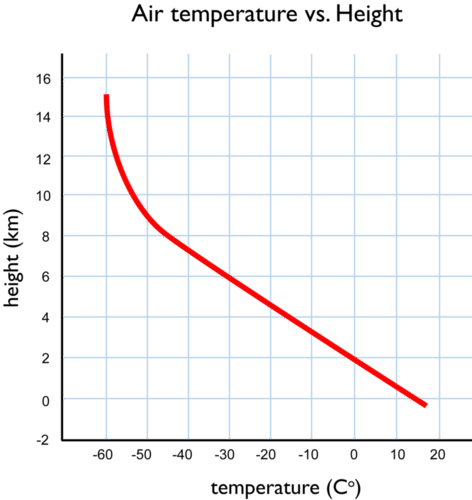
\includegraphics[width=0.6\textwidth]{img/tempvsheight.png}
        \centering
        \caption{Varion of temperature with respect to the height}
        \label{fig:tempvsheight}
    \end{figure}
\end{minipage}
\begin{minipage}[c]{0.6\textwidth}
    One of the main motivations behind causal analysis is a property called \textbf{similability}, 
    the ability o easily predict the output, given only any possible input.
\end{minipage}\\


We will consider causal analysis and discovery for time series since typically, 
input and output of a system are temporal signals, and we are interested in understanding 
how the system evolves and behaves over time.
This means, we want to understand how the temporal evolution of the output signal is affected
by the input signal (\textbf{and discovering which one is the input}).
We will denote as $V_T$ a variable $V$ which is observed for a temporal horizon $T$ (either continuous or
discrete)
\subsection{Structural causal model}
\begin{equation}
    V_t^j \coloneqq \textcolor{red}{f^j}(\textcolor{blue}{pa(V^j_t)}, \eta^j_t)\quad\text{for all }V_t^j\in \bm{V_t} \text{ and } t\in\mathbb{Z}
\end{equation}
Where $\textcolor{red}{f^j}$ is a generic non linear function, $\textcolor{blue}{pa(V^j_t)}$ are the parents of the variable $V^j$ i.e its causes and
$\eta^j_t$ is noise which comes from the uncertanty of the model or of the measurements.
\subsection{Granger's definition of causality (1969)}\label{sec:granger}
Given (temporal) variables $X$ and $Y$, we say that $X\;Granger-causes\;Y$
if $X$ contains information which affects $Y$ at time t, and such
information is not contained in the past of the universe ($Y$'s past or
other variables'past). In other words $Y$ depens \textbf{only} on $X$ and no other variables.If we only consider $Y$, we refer to bivariate causality \\

Granger's definition can be written in the following way as an autoregressive process:
\begin{equation}
    \bm{x_t}=\sum_{\tau=1}^{\tau_{max}}\phi(\tau)\bm{x}_{t-\tau}+\eta_t
\end{equation}
This formulation implies causality in mean (autoregressive model), this 
is a problem since it does not capture information about the distribution of the data.

\subsection{Conditional Mutual Information}
A more general definition comes from Schreibe: (bivariate) transfer entropy
\begin{equation}
    I^{TEbiv}_{X\rightarrow Y}=I(X_t^-;Y_t|Y_t^-)
    \label{eq:tebiv}
\end{equation}
where the `-` indicates the past of the variable and $I(X;Y|Z)$ denotes the Conditional Mutual Information (CMI).

\begin{equation}
    I(X;Y|Z)=\iiint{p(x,y,z)\log_2{\frac{p(x, y| z)}{p(x|z)\cdot p(y|z)}}dx\;dy\;dz}
    \label{eq:cmi}
\end{equation}
CMI (also called Related Entropy) comes from the concept of KL(Kullback-Leibler) divergence.
\begin{equation}
    D(p||q)=\sum_{x\in\mathcal{X}}p(x)\log{\frac{p(x)}{q(x)}}
\end{equation}
The KL divergence measures the degree of similarity between two distribution namely $p$ and $q$.
Similarly Mutual Information (MI) measures the discrepancy between joint distribution and the product of individual distributions.
Mutual Information(MI) is the same as CMI (eq \ref{eq:cmi}) but without the conditioning on $z$, so for the dicrete case the equation is:
\begin{equation}\label{eq:mi_disc}
    \begin{split}
        I(X;Y)&=\sum_{x\in\mathcal{X}}\sum_{y\in\mathcal{Y}}p(x,y)\cdot\log{\frac{p(x,y)}{p(x)p(y)}}\\
        &=D(p(x,y)||p(x)p(y))
    \end{split}
\end{equation}
This means that we can see MI as the KL divergence between the joint distribution and the product distribution.

\begin{tcolorbox}[colbacktitle=black!7!white,coltitle=black!75!white,title=\textbf{Statistics Recall}]
Let's make a quick statistics recall:\\
Given two random variables $x$ and $y$ if $x \text{ \textbf{indipendent}of } y$\\
$p(x,y) = p(x)p(y)$ so the product distribution is equal to the joint distribution\\\\
Given two random variables $x$ and $y$ if $x \text{ \textbf{dependent }on } y$\\
$p(x,y)=p(y)\cdot p(x|y)$
\end{tcolorbox}

So with MI we are trying to check if $x$ and $y$ are dependent:\\

\begin{center}
    \begin{minipage}[t]{0.4\textwidth}
        \noindent
        Assume $x$ and $y$ are \textit{\textbf{independent}}:
        \begin{equation}
            \begin{split}
                I(X;Y)&=\sum_{x\in\mathcal{X}}\sum_{y\in\mathcal{Y}}p(x,y)\cdot\log{\frac{\textcolor{red}{p(x,y)}}{p(x)p(y)}}\\
                &=\sum_{x\in\mathcal{X}}\sum_{y\in\mathcal{Y}}p(x,y)\cdot\log{\frac{\textcolor{red}{p(x)p(y)}}{p(x)p(y)}}\\
                &=\sum_{x\in\mathcal{X}}\sum_{y\in\mathcal{Y}}p(x,y)\cdot\log{\cancel{\frac{p(x)p(y)}{p(x)p(y)}}}\\
                &=\sum_{x\in\mathcal{X}}\sum_{y\in\mathcal{Y}}p(x,y)\cdot\log{1}\\
                &=\sum_{x\in\mathcal{X}}\sum_{y\in\mathcal{Y}}p(x,y)\cdot0\\
                &=0
            \end{split}
        \end{equation}
    \end{minipage}
    \begin{minipage}[t]{0.4\textwidth}
        \noindent
        Assume $x$ and $y$ are \textit{\textbf{dependent}}:
        \begin{equation}
            \begin{split}
                I(X;Y)&=\sum_{x\in\mathcal{X}}\sum_{y\in\mathcal{Y}}p(x,y)\cdot\log{\frac{\textcolor{red}{p(x,y)}}{p(x)p(y)}}\\
                &=\sum_{x\in\mathcal{X}}\sum_{y\in\mathcal{Y}}p(x,y)\cdot\log{\frac{\textcolor{red}{p(y)p(x|y)}}{p(x)p(y)}}\\
                &=\sum_{x\in\mathcal{X}}\sum_{y\in\mathcal{Y}}p(x,y)\cdot\log{\frac{\cancel{p(y)}p(x|y)}{p(x)\cancel{p(y)}}}\\
                &=\sum_{x\in\mathcal{X}}\sum_{y\in\mathcal{Y}}p(x,y)\cdot\log{\frac{p(x|y)}{p(x)}}\\
                &\ne 0
            \end{split}
        \end{equation}
    \end{minipage}
\end{center}
\newpage
So to recap:
\begin{itemize}
    \item $x \text{ and } y$ DEPENDANT$\rightarrow\;MI\ne 0$
    \item $x \text{ and } y$ INDIPENDENT$\rightarrow\;MI=0$
\end{itemize}
CMI(Eq \ref{eq:cmi}) is essentially the same but we measure if two variables are dependent given that both are conditioned by a third variable.
In other words given $x,y \text{ and } z$ how much $x$ and $y$ are indipendent given that both depend on $z$.
Differently from Granger Causality (Section \ref{sec:granger}) in MI and CMI 
we are evaluating the entire distribution instead of only the mean so it is 
more informative.\\
Given the above definition we can generalize the Granger formulation to include CMI:\\
$I^{FullCI}_{i\rightarrow j}(\tau)=I(X^i_{t-\tau};X^j_t|\bm{X}_t^{(t-1,\ldots,t-\tau_{max})}\setminus\{X^i_{t-\tau}\})$ 
\\here $\bm{X}_t^{(t-1,\ldots,t-\tau_{max})}$ is what we called $Z$ before i.e the past of all the variables.\\

To better understand causasality we can visualize it as a graph:
\begin{figure}[H]
    \centering
    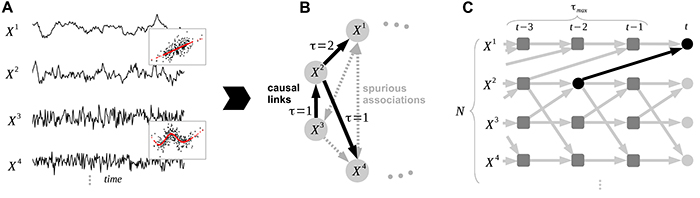
\includegraphics[width=0.8\textwidth]{img/visualization.jpeg}
\end{figure}
Consider a time series dataset (panel A) from a complex system of which we try to reconstruct the underlying causal dependencies (panel B), 
accounting for linear and nonlinear dependencies and including their time lags (link labels). 
